\documentclass{article}
\usepackage{graphicx}
\usepackage{hyperref}
\graphicspath{ {./images/} }
%Includes References in the table of contents%
\usepackage[nottoc]{tocbibind}

\usepackage[square, numbers]{natbib}
\bibliographystyle{abbrvnat}


\title{Team 26: Text summarization}



\begin{document}
	
\maketitle

\begin{abstract}
\noindent
	In our project, we have decided to create text summarizer with BERT. 
	There is already a Bert Extractive Summarizer -package. It's based on following article: \href{https://arxiv.org/ftp/arxiv/papers/1906/1906.04165.pdf}{https://arxiv.org/ftp/arxiv/papers/1906/1906.04165.pdf}
	This package is intended for lecture-summarization, and our goal is to extend and fine-tune this model for news or scientific articles.
	Even though foundational work is already done for the package, there's still much to customize such as tokenizer and model. 
	Our target language is english. Summarization tools such as Bilingual Evaluation Understudy (BLEU) and Recall-Oriented Understudy for Gisting Evaluation (ROUGE) are available, and part of the project is to try to evaluate the texts automatically and manually.	
\end{abstract}

\clearpage
\section{Introduction}
Automatic summarization is the process of shortening a set of data computationally, to create a subset (a summary) that represents the most important or relevant information within the original content. There are two main approaches to automatic summarization (independently of the application domain, e.g. text, images, video etc.):
\begin{itemize}
	\item Extraction-based or extractive summarization 
	\item Abstraction-based or abstractive summarization
\end{itemize}

When it comes to text documents, summarization is closely related to data compression and information understanding. The ability to produce coherent, well-structured summaries has the potential to transform efficiently the way that discovery systems work, as well as help human readers in skimming large datasets of text documents. That is why automatic summarization is considered one of the most important, yet least solved, tasks in NLP and a method that will transform the way people consume information on the Internet. In conclusion, applying text summarization reduces reading time, accelerates information retrieval and increases the amount of useful, dense information. In our case, we will deal with extractive summarization where a system produces summaries by choosing a subset of the initial text.

\section{Background}
The first summarization techniques go back already more than 50 years to Luhn’s and Edmundson’s seminal papers on automatic summarization (1958 and 1969 respectively, \cite{textmining1958}, \cite{automaticextracting}). Early work in the field dealt with single document summarization (news story, scientific articles etc.) Later, multi document summarization was applied in big data clusters to provide a coherent and brief digest to the users. \\

\noindent
A typical flow of an abstractive summarization system \cite{summarizing} consists of:
\begin{itemize}
	\item Interpretation to obtain an intermediate representation
	\item Transformation into a summary representation (sentence-level ranking)
	\item Generation based on semantically important sentences
\end{itemize}

A significant part of the intermediate representation is finding the most representative words of the text. The most common topic representation approaches \cite{survey} include:
\begin{itemize}
	\item Topic words 
	\item Frequency-based approaches (TF-IDF, word probability)
	\item Latent Semantic Analysis (LSA)
	\item Bayesian Topic Models (LDA)
\end{itemize}

Lately, neural modeling and huge pre-trained models have dominated the field \cite{neuralextractive}.

\section{BERT }
In many NLP tasks, the shortage of training data is often the source of the problems. There has been some research to tackle this issue by using unannotated text on the internet for training language representation models that serve general purpose. This process is also known as pre-training. The idea is that the pre-trained model can be fine-tuned later on small-data NLP tasks like question answering and sentiment analysis to have significant accuracy improvements compared to training on these datasets from scratch. 

BERT, also known as Bidirectional Encoder Representations from Transformers, is an example of pre-trained language representation models which uses a combination of masked language modeling objective and next sentence prediction on a large plain text corpus including Wikipedia and the Toronto Book Corpus. Unlike other language representation models, BERT is designed bidirectional in the way that it reads the input sequences. This characteristic allows the model to learn the context of a word from both left and right sides, capturing the previous and next contexts. BERT can also be fine tuned with one additional output layer to create state-of-the-art models for a wide range of tasks, such as question answering and language inference, without substantial task-specific architecture modifications. \cite{devlin2019bert}

\begin{figure}[h]
	\centering
	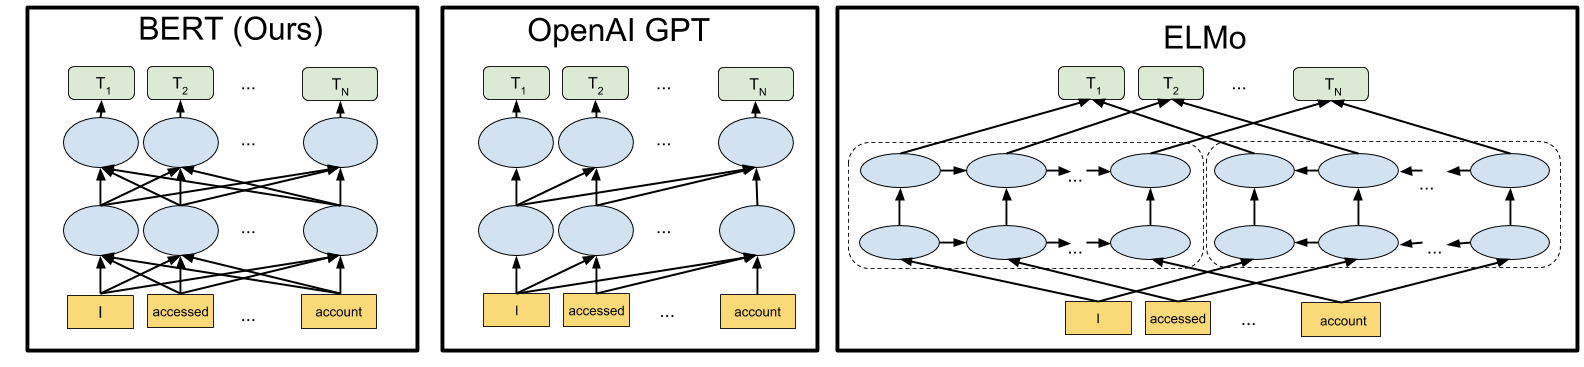
\includegraphics[scale=0.2]{image3.png}
	\caption{Architectures of known pre-training methods}
	\label{fig:mesh1}
\end{figure}

In the above figure created by Google AI, the neural network architectures state-of-the-art contextual pre-training methods are shown. The arrows show the information flow through layers while the green boxes indicate the final contextualized representation for input words. It can be seen that BERT is deeply bidirectional while OpenAI's GPT is unidirectional and ELMo has a shallow bidirectional structure.

BERT can also be considered conceptually simple. As mentioned earlier, BERT uses the advantage of bidirectionality by using a masked language modeling objective. Some words in the input text are masked out and each word are conditioned bidirectionally to predict the those masked words. It also uses next sentence prediction in which the model predicts if a sentence logically follows another sentence which was given previously. This task enables BERT to capture the relationship between sentences. \cite{devlin2019bert}

BERT has also been used in previous work for text summarization for news. In his paper, Yang suggests a fine tuned variant of BERT called BERTSUM for extractive summarization in which the input sequence and embeddings of BERT are modified to make it possible for extracting summaries. It is concluded that BERTSUM with inter-sentence Transformer layers achieve the best performance for extractive summarization of news, using CNN/DailyMail news and New York Times Annotated Corpus. \cite{liu2019finetune}

\section{The dataset}

The Cornell University NEWSROOM dataset \cite{dataset} consists of 1.3 million news articles and summaries between the years 1998 and 2017. It contains articles from 38 major publications and the summarization strategies combine both extraction and abstraction. The Newsroom website (summari.es) contains various different tools for analyzing the large article database. The dataset is written by humans with purpose of summarization. Dataset was created by scraping the website for content and using summaries in the HTML metadata. These metadata summaries were created to be found from search engines and social medias. Top news websites gathered from Alexa.com were used. \\

\noindent
We will be filtering the dataset \cite{dataset} to use extractive summaries, as our model is extractive. Another option for training dataset would be the New York Times corpus, which contains over 650 000 manually summarized news articles. These summarizations were done afterwards by library scientists. \cite{ny_dataset} 


\section{State of art }

Often, for the baseline precision Lede-3 is used. It's automatic summarization strategy that copies first $n$ words of the first sentence and uses it as summary. In our work we will be using this as a baseline also. Current state of art models in text summarization can be classified to fully extractive, fully abstractive or mixed models. In the study \cite{dataset} ROUGE-1, ROUGE-2 and ROUGE-L $F_1$ score variants were used to account for different summary lengths. In our work we will also be using ROUGE and BLEU scores for testing. We can test on both datasets \cite{dataset} \cite{ny_dataset}\\

\noindent
In the leaderboard it seems that mixed models perform the best, then comes the extractive and abstractive is the least efficient. TextRank was one of the best models in the study \cite{dataset} and it will also be used as comparison for our model.
The very least goal is to achieve better results than the Lede-3, but it will be interesting to see how well the extractive BERT performs ranks compared to TextRank. 

\section{Project plan}

We will be using Google Colabs resources for computing. It's convenient because we can store data in common cloud space, Google Drive, and Colab has a lot of computing power. We will be using BERT Extractive Summarizer -package for the actual modeling. The training data will be extractive data filtered from the NEWSROOM dataset \cite{dataset}. For evaluation, we will be using ROUGE and BLEU scores with the NEWSROOM dataset, and possible also New York Times Corpus dataset \cite{ny_dataset}. We will be comparing our result with the previously mentioned baseline Lede-3, and possibly also to more advanced TextRank. 

% Import bibliography file %
\bibliography{citations/sources.bib}


\end{document}